\documentclass{article}
\usepackage[utf8]{inputenc}
\usepackage[margin=0.625in]{geometry}
\usepackage{parskip, setspace}
\setstretch{1.15}
\usepackage{amsmath, amsfonts}
%\numberwithin{equation}{subsection}
\usepackage{graphicx, caption, wrapfig}
\usepackage{hyperref}
\usepackage{multirow}

\usepackage[ruled]{algorithm2e}

\usepackage{biblatex}
\addbibresource{bib.bib}

\renewcommand{\arraystretch}{1.5}

\title{\Large \vspace{-0.5in} CS 530: High-Performance Computing \\ Benchmarking Matrix Multiplication: Sequential vs Multithreaded \vspace{-0.25in}}
\author{Nathan Chapman \vspace{-0.05in} \\ \normalsize Department of Computer Science \vspace{-0.15in} \\ \normalsize Central Washington University}
\date{\normalsize \vspace{-0.15in}\today}

\begin{document}

\maketitle
\tableofcontents

\section{Introduction}

    There are many applications which can greatly benefit from being executed in parallel.  The ``best'' of these are those that are ``embarissingly parallel'', in which no data needs to be shared between threads.  One such context is that of matrix multiplication.  Matrix multiplication and matrix powers also serve as an excellent cases on which to highlight the differences that can be gained from parallel execution compared to sequential.

    Parallelism as it is normally implemented for a task such as matrix multiplication comes in the form of \emph{multithreading}.  Multithreading is the act of implementing a program in such a way that it makes use of the extra processing units in the CPU at the same time.  There is also multi-\emph{processing}, which is out of the scope of this investigation, but otherwise requires the use of message passing between different regions in memory.

\section{Methods}

    While there is support for the manual creation and management of threads in C with \verb|pthread_create| and \verb|pthread_join|, the Julia programming language natively supports creating thread pools when starting the Julia runtime process with \verb|julia -t n|, where \verb|n| is the number of threads to created in the thread pool.  Additionally, Julia can automatically assign tasks in a \verb|for| loop to its different threads with the use of OpenMP-pragma-like macros such as \verb|Threads.@threads|.  For example, a matrix multiplication parallelized over the rows of the product matrix can be seen in algorithm \ref{alg:parallelMatrixMultiplication}.  Further detail and examples can be found in the source code bundled with this report.

    \begin{algorithm}[h]
        \caption{Row-parallelized matrix multiplication using Julia's \texttt{Threads.@threads}}
        \KwIn{$N\times L$ Matrix A, $L \times M$ Matrix B}
        \KwOut{Matrix C of zeros}
        \texttt{Threads.@threads} \For{i $\in \{1, 2, \ldots, N\}$}{
            \For{j $\in \{1, 2, \ldots, M\}$}{
                \For{k $\in \{1, 2, \ldots, L\}$}{
                    C[i,j] $\gets$ C[i,j] + A[i, k] $\times$ B[k, j]
                }
            }
        }
        \label{alg:parallelMatrixMultiplication}
    \end{algorithm}

    In the representation shown in algorithm \ref{alg:parallelMatrixMultiplication} it can be seen that the runtime complexity of this implementation is reduced from the traditional implementation of matrix multiplication as $O(N^3)$ to $O(N^2)$.  This simplication comes from the fact that, while there are still $N$ column calculations that need to be considered, each with $N$ terms needing to be added together, these $N^2$ calculations are done at the same time, effectively transforming the outer-most $N$ operations in a factor of simply 1. Table \ref{tbl:runtimeComplexity} shows the associated runtime complexities for other forms of parallelized matrix multiplication.
    
    \begin{table}[h]
        \centering
        \begin{tabular}{|c||c|c|c|c|c|}
            \hline
            Parallelism & Rows & Columns & Summands & Complexity & Power Complexity \\
            \hline
            \hline
            Sequential & $N$  & $N$     & $N$      & $O(N^3)$    & $O(p N^3)$   \\
            \hline
            Row    & $1$  & $N$     & $N$      & $O(N^2)$        & $O(p N^2)$   \\
            \hline
            Column & $N$  & $1$     & $N$      & $O(N^2)$        & $O(p N^2)$   \\
            \hline
            Element & $1$  & $1$    & $N$      & $O(N)$          & $O(p N)$   \\
            \hline
        \end{tabular}
        \caption{Different runtime complexities for different levels of paralleism in matrix multiplication.}
        \label{tbl:runtimeComplexity}
    \end{table}

    For any form of parallelism (none, row, column, or element), when considering the \emph{power} $p$ of a matrix, the runtime complexity is simply linearly scaled by $p$.  This additional linear factor arises from each \verb|for| loop needing to be evaluated $p$ times, essentially creating another \verb|for| loop in $p$.  Algorithm \ref{alg:parallelMatrixPower} shows how algorithm \ref{alg:parallelMatrixMultiplication} can be modified to yield the power of matrix, while also highlighting how the runtime complexity changes.

    \begin{algorithm}[h!]
        \caption{Row-parallelized matrix power using Julia's \texttt{Threads.@threads}}
        \KwIn{$N\times N$ Matrix A, Power $P$}
        \KwOut{Matrix C of zeros}
        \For{p $\in \{1, 2, \ldots, P\}$}{
            \texttt{Threads.@threads} \For{i $\in \{1, 2, \ldots, N\}$}{
                \For{j $\in \{1, 2, \ldots, N\}$}{
                    \For{k $\in \{1, 2, \ldots, N\}$}{
                        C[i,j] $\gets$ C[i,j] + A[i, k] $\times$ B[k, j]
                    }
                }
            }
        }
        \label{alg:parallelMatrixPower}
    \end{algorithm}

    Finally, the results shown here are using the \verb|@elapsed| macro in Julia.  The \verb|time()| function, as it is in C, was also used but did not show differnt results.

\section{Results}

    Figures (\ref{fig:small_dim}, \ref{fig:med_dim}, \ref{fig:big_dim}) show the timings of matrix powers for different regions of the dimension-power space.  Figure (\ref{fig:small_dim}) shows the comparison between the sequential and paralleized matrix powers for different forms such as element-wise parallelism, row-wise, and column-wise.  Additionally, the relative timings, as compared to the sequential execution, are also displayed for comparison.  The other figures follow the same scheme.

    \begin{figure}[h]
        \centering
        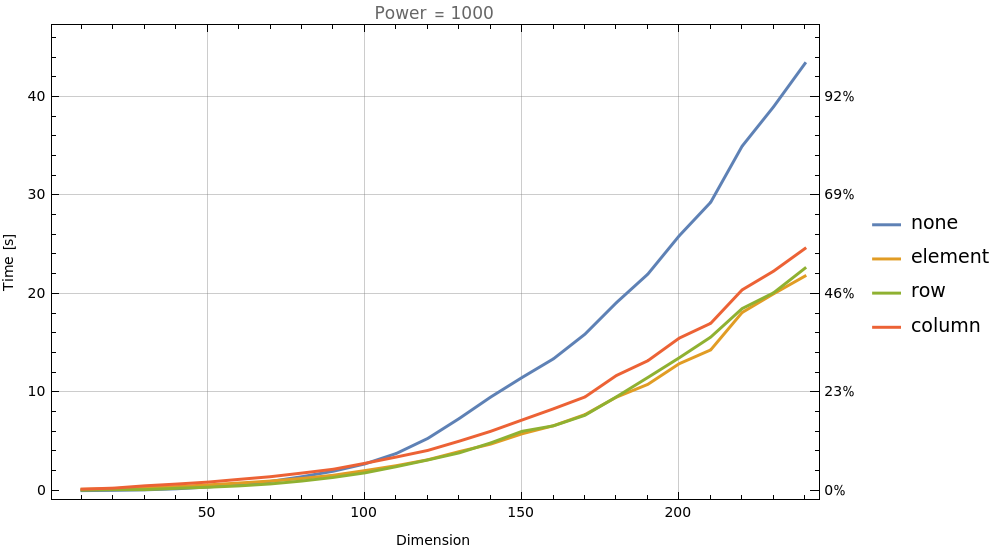
\includegraphics[width=0.75\textwidth]{images/dimension_small.png}
        \caption{Benchmarking for different forms of parallelism over matrix dimension, and a power of 1000.}
        \label{fig:small_dim}
    \end{figure}

    \begin{figure}[h!]
        \centering
        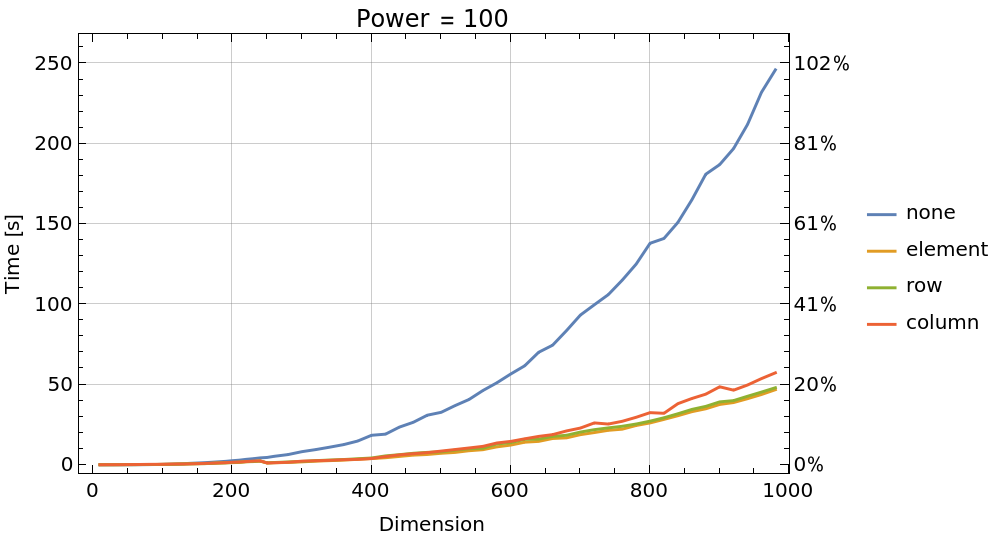
\includegraphics[width=0.75\textwidth]{images/dimension.png}
        \caption{Benchmarking for different forms of parallelism over matrix dimension, and a power of 100}
        \label{fig:med_dim}
    \end{figure}

    \begin{figure}[h!]
        \centering
        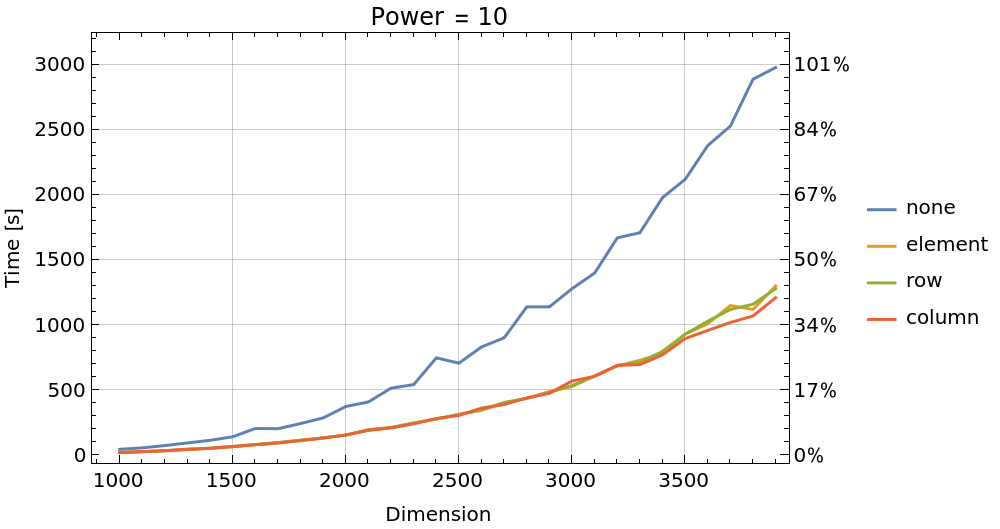
\includegraphics[width=0.75\textwidth]{images/big_dim.png}
        \caption{Benchmarking for different forms of parallelism over large matrix dimensions, and a power of 10}
        \label{fig:big_dim}
    \end{figure}

    Figure (\ref{fig:power}) shows how the execution time of the paralleized matrix power depends on the power to which the matrix is raised.

    \begin{figure}[h]
        \centering
        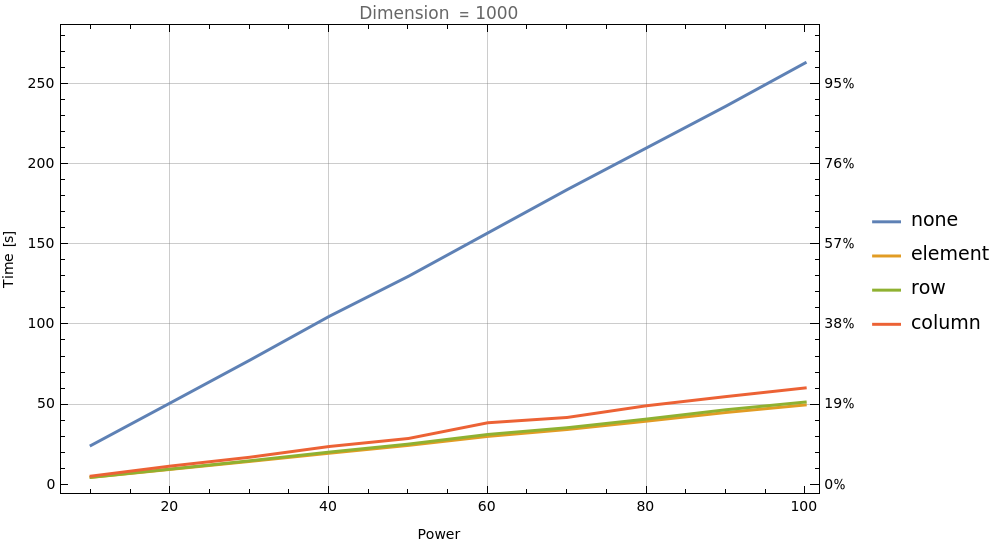
\includegraphics[width=0.75\textwidth]{images/power.png}
        \caption{Benchmarking for different forms of parallelism over large matrix dimensions, and a power of 10}
        \label{fig:power}
    \end{figure}

    The results in figures (\ref{fig:med_dim}, \ref{fig:power}, \ref{fig:small_dim}) were gathered on a machine with the specifications shown in table \ref{tbl:homeSpecs}, while the results in figure (\ref{fig:big_dim}) were gathered on a machine with specifications as show in table (\ref{tbl:officeSpecs}). 

    \begin{table}[h!]
        \centering
        \begin{tabular}{|c||c|c|c|c|c|}
            \hline
            OS & Manjaro Linux \\
            \hline
            Kernel & Linux 6.6.30-2-MANJARO \\
            \hline
            Shell & bash 5.2.26 \\
            \hline
            CPU & 13th Gen Intel i7-13700K (24) @ 5.3GHz \\
            \hline
            GPU & NVIDIA GeForce RTX 3060 Ti Lite Hash Rate \\
            \hline
            Memory & 31.18GiB  \\
            \hline
            GPU Driver & NVIDIA 550.78 \\
            \hline
        \end{tabular}
        \caption{Different runtime complexities for different levels of paralleism in matrix multiplication.}
        \label{tbl:homeSpecs}
    \end{table}

    \begin{table}[h!]
        \centering
        \begin{tabular}{|c||c|c|c|c|c|}
            \hline
            OS & Arch Linux \\
            \hline
            Kernel & Linux 6.6.30-2 \\
            \hline
            Shell & bash 5.2.26 \\
            \hline
            CPU & 6th Gen Intel i5-6500 (4) @ 3.2GHz \\
            \hline
            GPU & NVIDIA GeForce GTX 1660 Super \\
            \hline
            Memory & 16GiB  \\
            \hline
        \end{tabular}
        \caption{Different runtime complexities for different levels of paralleism in matrix multiplication.}
        \label{tbl:officeSpecs}
    \end{table}

    \clearpage
    \pagebreak
\section{Discussion}
    
    While each figure could not more clearly suggest that using multiple threads to execute matrix multiplications results in drastically smaller execution times, there are discrepancies between them.  When considering matrices with a ``medium'' dimension as in figure (\ref{fig:med_dim}), the execution time of multiplication is quite staggering at around an 80\% reduction in execution time.  This is in contrast to the timings found for ``small'' matrices as in figure (\ref{fig:small_dim}) where there was only a reduction of around 50\%.  Assuming this trend continues, one should assume the timings for ``large'' matrices (as in figure (\ref{fig:big_dim})) should yield an even larger reduction in execution time.  Figure (\ref{fig:big_dim}) though does not show a consistency in this trend, only showing a reduction by about 50\%.  There could be many factors causing this discrepancy, but most notably is the use of a different machine.  The large-matrix timings were found on a machine with specifications as shown in table (\ref{tbl:officeSpecs}), whereas the other results were found on a machine with specifications as shown in figure (\ref{tbl:homeSpecs}).  The most relevant difference between these two machines is the number of cores in the CPU: the large-matrix machine only used 4 cores and 4 threads at 3.2 GHz while the medium-matrix machine used 20 cores with 20 threads at 5.2 GHz.  In order to accurately extrapolate a trend for these results, the large-matrix timings would need to be evaluated on the same machine as the small- and medium-matrix results.  
    
    The results in each of varying-dimension cases are consistent with the prediction that the execution time of sequential matrix powers depends cubically on the dimension of the matrix.  Likewise, the execution time of matrix powers when evaluated in row- or column-wise parallel depends quadratically on the dimension of the matrix.  As for element-wise parallelism, the prediction is that the execution time should scale linearly (assuming there is a core for every thread), but each of the dimension figures (\ref{fig:small_dim}, \ref{fig:med_dim}, \ref{fig:big_dim}) all show the execution time of the element-wise parallelism to match with the row- and column-wise results.  This discrepancy between the prediction and experiment certainly warrants further investigation.  The results as shown in figure (\ref{fig:power}) are consistent with the prediction at the execution time of matrix powers should increase linearly with the power.

\section{Conclusion}

    Many applications can benefit from being executed in parallel over multiple threads.  A subset of these applications require the use of \emph{many} threads in order to execute in a reasonable time.  Low level approaches like C's \verb|pthread_create|, \verb|pthread_join|, etc. are excellent resources when the need arises to have direct control over the creation, synchronization, and management of threads on a near hardware level.  This capability, though not using pthreads, is further highlighted when using massively parallel architecture such as a GPU with the CUDA parallel computing framework.  For other applications, a higher level approach, such as using Julia, is sufficient and allows for more rapid development with minimal introduced execution overhead.

    Some of the aforementioned applications are so-called ``embarissingly parallel'', such as matrix multiplication.  It is in these applications that creating multithreaded algorithms and implementations is easy.  Other applications, namely those in which the threads need to share data by either reading or writing concurrently, require much more sophisticated approaches utilizing tools such as mutex locks or atomic variables.  Though when done properly, the extra work can lead to massive reduction in execution time.

    By far and away, the most substantial effect parallelism has on an execution is the massive reduction in exeuction time.  As with matrix multiplication, the differences between a sequential implementation and a parallel implementation could lead to 80\% reduction in computation time.  For example, in the case of considering an autonomous vehicle, it would be best for the instructions to be evaluated in parallel so in the case where a pedestrian is in the way, there is minimal time between the machine gathering the data, evaluting, and stopping.  Other applications, such as evaluating the terms of the Fibonacci sequence would not benefit from parallelism because it is inherently a recursive algorithm and thus must be done sequentially.  Ultimately, there are many applications where the use of parallelism would greatly (80\%!) reduce the time it takes to yield a result, but there are many others where paralleism is impossible.

\end{document}